\setcounter{chapter}{-1}
\chapter{Preliminaries}

\section{Geometric Structures on Manifolds}
\textbf{TODO: Basic definitions of (G,X)-structures}
\begin{prop}
    Let $M$ be a simply connected $(G,X)$-manifold. Then there exists a $(G,X)$-map
    $$
        dev: M \mapsto X
    $$
\end{prop}
\begin{proof}
    We pick a base point $x_0 \in M$ and a chart $(U_0, \varphi_0)$ around $x_0$. Now for any $x \in M$ we define the map $dev$ as follows. We pick a curve on $M$ $x(t)$ satisfying $x(0)=x_0$ and $x(1)=x$. As the image of our curve is compact, we can cover the it by finitely many coordinate charts $U_i$ with $i\in \{0, \dots,n\}$ such that $x(t) \in U_i$ for $t\in(a_i, b_i)$ with
    $$a_0<0<a_1<b_0<a_2<b_1<a_3 \dots <a_n<b_{n-1}<1<b_n$$

    \begin{center}
        \begin{marginfigure}
            \vspace{8px}
            \centering
            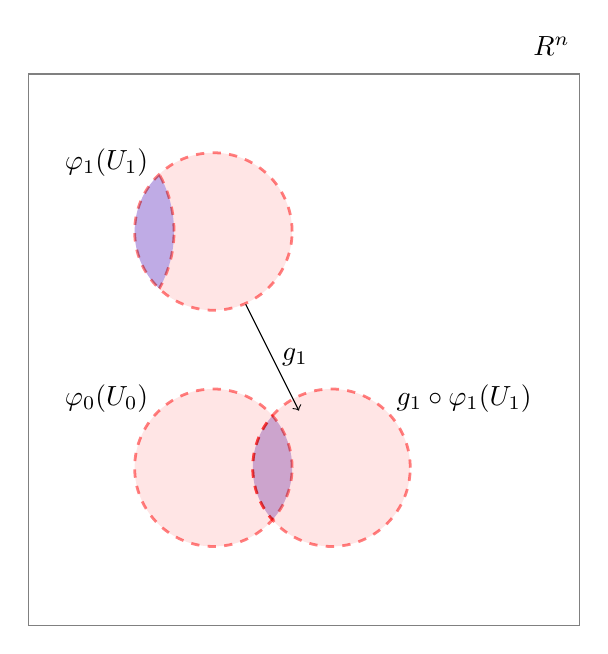
\begin{tikzpicture}
                \begin{scope}
                    \begin{scope}
                        \draw[color=black!50] (0,0) rectangle (7,7) node[color=black,anchor=east, yshift=10pt]{$\mathbb{R}^n$};
                    \end{scope}
                    \begin{scope}[transparency group]
                        \begin{scope}[blend mode=multiply, yshift=10cm, xshift=10pt]
                            \draw[dashed, color=red!50!white, fill=red!10, opacity=1]
                            (2,-8) circle (1) node[anchor=east, xshift=-20pt, yshift = 25pt, color=black]{$\varphi_0(U_0)$};
                            \draw[dashed, color=red!50!white, fill=red!10,opacity=1] (2, -5) circle (1) node[anchor=east, xshift=-20pt, yshift = 25pt, color=black]{$\varphi_1(U_1)$};
                            \begin{scope}
                                \clip (2, -5) circle (1);
                                \draw[dashed, color=red!50!white, fill=blue!25, opacity=1]
                                (0,-5) circle (1.5);
                            \end{scope}

                            \begin{scope}
                                \clip (2, -8) circle (1);
                                \draw[dashed, color=red!50!white, fill=blue!20,opacity=1] (3.5, -8) circle (1);
                            \end{scope}
                            \draw[dashed, color=red!50!white, fill=red!10,opacity=1] (3.5, -8) circle (1) node[anchor=west, xshift=20pt, yshift = 25pt, color=black]{$g_1 \circ \varphi_1(U_1)$};

                        \end{scope}
                    \end{scope}
                    \node[] (GluingOneTwoStart) at (2.7,4.2) {};
                    \node[] (GluingOneTwoEnd) at (3.5,2.6) {};
                    \path[->]
                    (GluingOneTwoStart) edge[right] node [midway, right] {$g_{1}$} (GluingOneTwoEnd);
                \end{scope}

            \end{tikzpicture}
            \caption{Gluing together charts}
            \label{fig:placeholder}
        \end{marginfigure}
        \begin{figure}[h]
            \centering
            \begin{tikzpicture}
                \begin{scope}[transparency group]
                    \begin{scope}[blend mode=multiply]
                        \draw[color=black!50] (0,0) rectangle (8,7) node[color=black,anchor=east, yshift=10pt]{\textbf{M}};
                        \draw[dashed, color=red!50!white, fill=red!10, opacity=1]
                        (1,1.8) circle (0.8) node[anchor=east, xshift=-10pt, yshift = 25pt, color=black]{$U_0$};
                        \draw[dashed, color=red!50!white, fill=red!10,opacity=1] (2, 2.5) circle (0.8) node[anchor=east, xshift=10pt, yshift = 30pt, color=black]{$U_1$};
                        \draw[-, dotted, thick] (2.8,3.5) arc (140:90:4cm and 3cm);
                        \draw[dashed, color=red!50!white, fill=red!10,opacity=1] (7, 4.7) circle (0.8) node[anchor=east, xshift=10pt, yshift = 30pt, color=black]{$U_n$};
                    \end{scope}
                \end{scope}
                \draw [cyan, yshift=-1.3cm, thick] plot [smooth, tension=1] coordinates { (1, 3) (3, 4.5) (6, 5) (7, 6)} node[color=black] at (4.5,4.5) {$x(t)$};
                \node[yshift=-1.3cm, draw, circle, fill=black!50, inner sep=1pt] (start) at (1,3) {} node[right = of start, xshift=-30pt, yshift=-5pt]{$x_0$};
                \node[yshift=-1.3cm, draw, circle, fill=black!50, inner sep=1pt] (end) at (7,6) {} node[right = of end, xshift=-30pt, yshift=-5pt]{$x$};
            \end{tikzpicture}
            \caption{Covering of $x(t)$ by charts}
            \label{fig:placeholder}
        \end{figure}
    \end{center}

    Now we consider where these charts overlap. Since our manifold is equipped with
    a $(G,X)$-structure our transition maps differ by an element of $G$. Let $g_i =
        \varphi_{i-1}\circ\varphi^{-1}_i \in G$ be the transition map from $U_i$ and
    $U_{i-1}$. We then define $$ dev(x) = g_1g_2\dots g_n \varphi_n(x) $$ We must
    show that this is a well-defined map. We first show that this map does not
    change if we refine the cover. Suppose we insert a chart $(V, \phi)$ between
    $U_i$ and $U_{i-1}$. Let
    \begin{center}
        $\varphi_{i-1} = h_{i-1}\circ\phi$ on $V \cap U_{i-1}$ and \\
        $\phi = h_i\varphi_{i}$ on $V \cap U_{i-1}$.
    \end{center}
    Then on $V \cap U_i \cap U_{i-1}$ we have that $\varphi_{i-1} = h_{i-1}\circ h_i \circ \varphi_{i}$. This gives us that $g_i = \varphi_{i-1}\circ \varphi^{-1}_i = h_{i-1} \circ h_i$ as we require that our transition maps satisfy a unique extension property.

    Now when we develop along our curve with respect to this new covering, we
    obtain that:

    \begin{center}
        $dev(x) = g_1 \dots g_{i-1}h_{i-1}h_{i}g_{i+1}\dots g_n\varphi_n(x) = g_1 \dots g_{i-1}g_ig_{i+1}\dots g_n\varphi_n(x)$
    \end{center}

    This defines $dev$ along $x(t)$. We now need to show that it does not depend on
    our choice of curve. As $M$ is simply connected, all curves with the same start
    point and end point will be homotopic. Indeed, by compactness we can split our
    homotopy into smaller homotopies such that we can break up our curve into
    regions
    \begin{center}
        $a_1 =0 < a_2 < \dots < a_n=1$
    \end{center}
    such that during each small homotopy the segment $x((a_i, a_{i+1}))$ lies entirely inside a coordinate patch. It then follows that $dev$ is independent of our choice of paths completing the proof.

\end{proof}

This shows that we have a well defined development map on any simply connected
$(G,X)$-manifold. However, this map depended on the choice of base point and
initial chart. We immediately get the following corrolary from this fact.

\begin{corollary}
    Let $M$ be a $(G,X)$-manifold and let $\tilde{M}$ be its universla cover. Then
    there exists a pair $(dev, hol)$ satisfying
    \begin{center}
        $dev : \tilde{M} \mapsto X$\\
        $hol: \pi_1(M) \mapsto G$
    \end{center}
    where $hol(\gamma)$ is the element $g_1\dots g_n$ of $G$ obtained from
    developing around a loop $\gamma \in M$.
\end{corollary}

The developing pair satisfy the following equivariance condition.
\begin{lemma}
    Let $\gamma, \alpha \in \pi_1(M)$ be loops in $M$. Then

    \begin{center}
        $dev(\gamma \star \alpha) = hol(\gamma)dev(\alpha)$
    \end{center}
\end{lemma}

\begin{proof}
    Let $\{(U_i, \varphi_i)\}$ be a cover for $\alpha$ and $\{(V_i, \phi_i)\}$ be
    cover for $\gamma$. Denote the transition maps on $U_i \cap U_{i+1}$ by $h_i$
    and the transition maps on $V_i \cap V_{i+1}$ by $g_i$. Then by definition
    \begin{center}
        $dev(\gamma \star \alpha) = g_1 \dots g_n h_1 \dots h_k \varphi_k(\alpha(1))$\\
        $= hol(\gamma)dev(\alpha)$
    \end{center}
\end{proof}

The role of the development pair is to "globalize" the coordinate chart of $M$.
Indeed the following proposition makes this statment more clear.

\begin{prop}
    Let $M$ be a $(G,X)$-manifold with development pair $(dev, hol)$. Denote
    by $\Gamma$, the image of $\pi_1(M)$ under the holonomy map. Then there
    exists a $(G,X)$-atlas such that the transition maps lie in $\Gamma$
\end{prop}

\begin{proof}
    We pick $m\in M$ and fix a lift $\tilde{m}\in \tilde{M}$ of $m$. Then, as
    $dev$ is a local diffeomorphism, there is an open set $\tilde{U}$ of $\tilde{m}$
    such that $dev$ is a local diffeomorphism onto $X$.

    We pick $V \subset M$ an open neighborhood of $m$ and take its inverse under
    the covering map $p^{-1}(V)$ which we may assume $dev$ is a diffeomorphism on
    by intersetcting with $\tilde{U}$.

    Now, define coordinate charts on $M$ by $(V_{\alpha}, \psi_{\alpha} = dev \circ
        p^{-1}_{\alpha})$ at a point $m \in M$ where by $p^{-1}_{\alpha}$ we mean we
    have fixed a component of the preimage $p^{-1}$ restricted to $V_{\alpha}$. Now
    suppose that $V_i \cap V_j \neq \emptyset$ and let $\tilde{U}_i =
        p_i^{-1}(V_i)$ and $\tilde{U}_j = p_j^{-1}(V_j)$. Then the preimage of their
    intersection will differ by a deck transformation $\gamma \in \pi_1(M)$.
    Therefore, on the intersection $V_i \cap V_j$
    \begin{center}
        $dev \circ p_i^{-1} = dev \circ \gamma \circ p_j^{-1}$\\
        $\implies p^{-1}_i \circ p_j = \gamma$
    \end{center}

    Now our by definition of our transition maps
    \begin{center}
        $\psi_i \circ \psi_j^{-1} = dev \circ p_i{-1} \circ p_j \circ dev^{-1}$\\
        $= dev \circ \gamma \circ dev^{-1} = hol(\gamma)dev\circ dev^{-1} = hol(\gamma) \in \Gamma$
    \end{center}

    and so we have thus given our coordinate charts on $M$ in terms of the
    development pair.
\end{proof}

This shows that once we have fixed a development pair, our $(G,X)$-structure is
entirely determined by this. Conversely, the following lemma shows us that Once
we have fixed our $(G,X)$-structure, the development pair is determined up to
certain factors/conjugations.

\begin{lemma}
    Let $M$ be a $(G,X)$-manifold with development pair $(dev, hol)$. Suppose that $(dev', hol')$ is
    another development pair for $M$. Then $dev' = g\circ dev$ and $hol' = g\circ hol \circ g^{-1}$
    for some $g \in G$
\end{lemma}
\begin{proof}
    Our development pair was determined once we picked a base point and a chart $(U, \phi)$. Suppose that
    we pick a different base point and chart $(V, \varphi)$. Now we consider how we define $dev(x)$ for $x \in \tilde{M}$.
    We choose a curve $\gamma$ connecting $x_0$ and $x$ and choose a cover $U_i$ of $\gamma$ and develop around it.
    Now, with respect to our new initial chart, $V \cup \{U_i\}$ is an open cover of $\gamma$. If we develop starting with this new chart,
    we can first glue all the $U_i$ to $U_1$ as before and then glue this chain to $V$ with an element of $G$ by gluing
    $U_1$ to $V$ on their overlap. Hence the entire development will have o=just changed by that element of $G$.

    If, on the other hand, both the base point and chart have changed, we can pick
    a curve $\gamma'$ starting at our new base point $x_0'$ and ending at our old
    basepoint $x_0$. Developing first along this curve and then along our old curve
    $\gamma$ we pick up some element of $G$ from developing $\gamma'$ whilst
    developing along $\gamma$ gives the same as before. As we already showed this
    map is homotopy invariant this gives that $dev'(x) = g\circ dev(x)$ for some $g
        \in G$.

    Now to show that $hol' = g\circ hol \circ g^{-1}$ we consider
    \begin{center}
        $dev'(\gamma \star \alpha) = g \circ dev(\gamma \star \alpha)$\\
        $= g\circ hol(\gamma) \circ dev(\alpha)$\\
        $= (g\circ hol(\gamma)\circ g^{-1})(g\circ dev(\alpha))$\\
        $= (g \circ hol(\gamma)\circ g^{-1})dev'(\alpha)$
    \end{center}
    and as the development pair satisfied the equivariance property it follows that
    $hol' = g\circ hol \circ g^{-1}$.
\end{proof}

This shows that once we have fixed a development pair, any other development
pair can is related by $(dev', hol') = (g\circ dev, g\circ hol \circ g^{-1})$.
It is therefore, important to note that if we want to classify
$(G,X)$-structures on a manifold $M$ by classifying the possible development
pairs, it is important to consider them up to this relation.

\subsection{Completeness}
An important property the developing map can have is that of
\textbf{completeness}.
\begin{definition}
    A $(G,X)$-manifold $M$ is said to be complete if its developing map is a diffeomorphism
    onto $X$.
\end{definition}
In the case that $X$ is simply connected e.g. $X= \mathbb{R}^n$, we have that $M$ is diffeomorphic
to $X/\Gamma$ where $\Gamma = hol(\pi_1(M))$.

In the case that $M$ is a Riemannian manifold, this notion of completeness is
equivalent to completeness of the Levi-Civita connection of $M$.

\textbf{TODO :
    Examples of complete/ incomplete manifolds e.g. Hopf}
\section{Representation Theory and Affine Manifolds}
We now turn our attention to affine manifolds before specializing to the
integral affine case. An affine manifold is a $(G,X)$-manifold where $X =
    \mathbb{R}^n$ and $G = Aff(\mathbb{R}^n)$ An important tool in classifying
affine structures is the representation theory of groups. Often, by studying
properties of the holonomy group of an affine manifold $M$, we are able to
obtain information about the affine structure of $M$. Of fundamental importance
is the case where the holonomy group is nilpotent which we will shortly see. We
will use these tools to determine conditions for which the affine structure is
complete.

\begin{definition}
    An affine transformation of $\mathbb{R}^n$ is a map
    \begin{center}
        $A: \mathbb{R}^n \mapsto \mathbb{R}^n$
    \end{center}
    such that $A(x) = Gx + B$ where $G \in GL(\mathbb{R}^n)$ and $B \in\mathbb{R}^n$
\end{definition}

The group $Aff(\mathbb{R}^n)$ is the group of affine transformations of
$\mathbb{R}^n$ and is equal to $Aff(\mathbb{R}^n) = \mathbb{R}^n \rtimes
    GL(\mathbb{R}^n )$

\begin{definition}
    An affine representation of a group $G$ is a group homomorphism
    \begin{center}
        $\alpha: G \mapsto Aff(\mathbb{R}^n)$
    \end{center}
\end{definition}

We have that an affine representation splits into a linear part and a
translation, e.g. $\alpha(g) = \lambda(g) + \mu(g)$. The linear part makes
$\mathbb{R}^n$ into a $G$-module with the obvious action which we will denote
$E$.

We will be interested in some results from group cohomology. This leads us to
the following definitions.

\begin{definition}[Crossed Homomorphism]
    A crossed homomorphism for $\lambda$, is a group homomorphism
    \begin{center}
        $\mu: G \mapsto E$
    \end{center}
    that satisfies $\mu(gh) = \mu(g) + \lambda(g)\mu(h)$
\end{definition}

\begin{prop}
    Let $\alpha(g) = \lambda(g) + \mu(g)$ be an affine representation on $E$ of a group G. Then
    $\mu$ is a crossed homomorphism for $\lambda$
\end{prop}
\begin{proof}
    Let $g,h \in G$ and $\alpha = \mu + \lambda$ be an affine representation. Then
    \begin{center}
        $\alpha(gh) = (\mu(gh), \lambda(gh))$\\
        $=\alpha(g)\cdot \alpha(h)= (\mu(g), \lambda(g)) \cdot(\mu(h), \lambda(h)) $\\
        $= (\mu(g) + \lambda(g)\mu(h), \lambda(g)\lambda(h))$\\
        $\implies \mu(gh) = \mu(g) + \lambda(g)\mu(h)$
    \end{center}
    and so $\mu$ is a crossed homomorphism for $\lambda$.
\end{proof}

\begin{definition}[Principle Crossed Homomorphism]
    A \textit{principle crossed homomorphism} for $\lambda$ is a crossed homomorphism
    of the form $\mu(g) = y- \lambda(g)y$ for some $y \in E$.
\end{definition}

\begin{prop}
    Let $y\in E$. Then y is a \textit{stationary point} of the action of $\alpha$ if
    and only if $\mu(g) = y - \lambda(g)y$ for all $g \in G$.
\end{prop}

\begin{proof}
    Suppose $y \in E$ is a stationary point of $\alpha$. Then $\alpha(g)y = y$ for every $g \in G$.
    This gives that
    \begin{center}
        $(\lambda(g) + \mu(g))y = \lambda(g)y + \mu(g) = y$\\
        $ \implies \mu(g) = y - \lambda(g)y$
    \end{center}

    Conversely, suppose that $\mu(g) = y - \lambda(g)y$. Then $y = \mu(g) +
        \lambda(g)y = \alpha(g)y$ \label{lemma:stationary}
\end{proof}
\begin{remark}
    If $\mu$ is a principle crossed homomorphism we will often write $\mu = D_y$
\end{remark}

\begin{remark}
    An affine representation with a fixed point is called \textit{radiant}.
\end{remark}

\textbf{TODO: Develop some of the basics of group cohomology}

\begin{lemma}
    The cohomology group $H^1(G, E)$ is isomorphic to
    \begin{center}
        $H^1(G,E) \cong \frac{\{\text{crossed homomorphisms for } \lambda\}}{\{\text{principle crossed homomorphisms for } \lambda\}}$
    \end{center}
\end{lemma}

\begin{proof}
    \textbf{TODO : Add proof e.g. construct resolution or take this as given?}
\end{proof}

\begin{definition}[Radiance Obstruction]
    Let $\alpha$ be an affine representation. The radiance obstruction of $\alpha$ is the cohomology
    class
    \begin{center}
        $c_{\alpha} = [\mu] \in H^1(G, E)$
    \end{center}
    where $\mu$ is the translational part of $\alpha$.
\end{definition}

\begin{lemma}
    The radiance obstruction vanishes, e.g. $c_{\alpha} = 0$ if and only if
    $\alpha$ is conjugate to its linear part by a translation, if and only if $\alpha$
    has a stationary point.
\end{lemma}
\begin{proof}
    By Lemma~\ref{lemma:stationary}, $y \in E$ is stationary if and only if
    $\mu(g) = D_y$ is a principle crossed homomorphism for $\lambda$ if and only
    if $c_{\alpha} = [\mu] =0$.

    Now suppose that $\mu =D_y$ for some $y \in E$. so that $\mu(g) = y -
        \lambda(g)y$. We define the translation
    \begin{center}
        $T_y : E \mapsto E$\\
        $ x \mapsto x-y$
    \end{center}
    Now, conjugating $\alpha$ by this translation yields
    \begin{center}
        $T_y \circ \alpha(g) \circ T_y^{-1} = T_y\circ \alpha(g)(x+y)$\\
        $= T_y\circ(\lambda(g)x  + \lambda(g)y + \mu(g))$\\
        $= T_y \circ (\lambda(g)x + \lambda(g)y +y - \lambda(g)y)$\\
        $= T_y \circ (\lambda(g)x +y ) = \lambda(g)x +y-y = \lambda(g)x$
    \end{center}

    Conversely, suppose that $T_y \circ \alpha(g) \circ T_y^{-1} = \lambda(g)$ for
    all $g \in G$ and $x \in E$. Then
    \begin{center}
        $T_y \circ \alpha(g) \circ T_y(x) = T_y \circ \alpha(g)(x+y)$\\
        $= T_y \circ (\lambda(g)(x+y) + \mu(g)) = \lambda(g)(x+y)+\mu(g)-y = \lambda(g)x$\\
        $\implies \mu(g) = \lambda(g)(x) - \lambda(g)(x) - \lambda(g)(y) +y$\\
        $= y - \lambda(g)y$
    \end{center}
    as required.
\end{proof}

\begin{remark}
    This lemma will allow us to alter the development map by a translation (which
    alters the holonomy representation by a conjugation) to assume that our fixed
    point is at the origin.
\end{remark}

